% =====================================================================
% Structured Belief Revision and the Dynamics of Paradigm Change
% Figure-driven companion to pomdp_paradigm_model.tex.
% A paradigm is a structured belief network whose nodes pass messages
% to neighbours in BOTH directions (input + output). A core belief
% structure and its higher conservatism are part of the update setup for
% the network, not read off the graph. Paradigm shifts appear as a
% percolation cascade from belt to core; a changed belief must then be
% communicated, which raises the question of what is transmitted.
% Compile: pdflatex structured_belief_revision   (self-contained, inline bib)
% =====================================================================
\documentclass[11pt,a4paper]{article}

\usepackage[T1]{fontenc}
\usepackage[utf8]{inputenc}
\usepackage[margin=1in]{geometry}
\usepackage{amsmath,amssymb,bm}
\usepackage{microtype}
\usepackage{xcolor}
\usepackage{tikz}
\usetikzlibrary{positioning,arrows.meta,calc,fit,backgrounds,shapes.geometric}
\usepackage{pgfplots}
\pgfplotsset{compat=1.18}
\usepackage[round,authoryear]{natbib}
\usepackage{hyperref}
\hypersetup{colorlinks=true,linkcolor=blue,citecolor=blue,urlcolor=blue}

% ---- colour semantics ------------------------------------------------
\definecolor{paradA}{HTML}{2166AC}  % old paradigm (belief value)
\definecolor{paradB}{HTML}{B2182B}  % new paradigm (belief value)
\definecolor{social}{HTML}{1B7837}  % communication / trust
\definecolor{util}{HTML}{D9730D}    % affective belief-utility
\definecolor{cons}{HTML}{5E3C99}    % conservatism shading ramp

\newcommand{\KL}[2]{D_{\mathrm{KL}}\!\left[#1\,\|\,#2\right]}
\newcommand{\E}[1]{\mathbb{E}\!\left[#1\right]}

% ---- node / edge styles ---------------------------------------------
\tikzset{
  bnode/.style ={circle, inner sep=0pt, font=\scriptsize},
  core/.style  ={bnode, minimum size=9mm, line width=1pt},
  periph/.style={bnode, minimum size=6mm, line width=0.5pt},
  old/.style   ={draw=paradA, fill=paradA!15},
  new/.style   ={draw=paradB, fill=paradB!22},
  % one directed message along an edge; pairs of these make a link bidirectional
  msg/.style   ={draw=gray!60, line width=0.4pt, -{Stealth[length=3pt]},
                 shorten >=1.5pt, shorten <=1.5pt},
  minilink/.style={draw=gray!55, line width=0.4pt,
                 {Stealth[length=2pt]}-{Stealth[length=2pt]}},
  obsq/.style  ={rectangle, draw=social, fill=social!12, minimum size=5mm,
                 inner sep=1pt, font=\scriptsize},
  agent/.style ={circle, draw=gray!70, fill=gray!4, minimum size=11mm,
                 line width=0.7pt},
  >=Stealth,
}

% A bidirectional link = two directed messages (input + output), one each way.
\newcommand{\biarrow}[2]{%
  \draw[msg] (#1) to[bend left=7] (#2);
  \draw[msg] (#2) to[bend left=7] (#1);}

% ---- the shared belief-network topology (16 nodes: 4 core + 12 belt) -
\def\corelist{A/0/0, B/2.4/0, C/0/-2.4, D/2.4/-2.4}
\def\periphlist{%
  pA1/-2.1/1.0/a_1, pA2/-0.4/1.9/a_2, pA3/-2.3/-0.6/a_3,
  pB1/2.8/1.9/, pB2/4.5/1.0/, pB3/4.7/-0.5/,
  pC1/-2.3/-1.8/, pC2/-2.1/-3.4/, pC3/-0.4/-4.3/,
  pD1/2.8/-4.3/, pD2/4.5/-3.4/, pD3/4.7/-1.9/}
\def\coreedges{A/B, A/C, B/D, C/D, A/D}
\def\periphedges{A/pA1, A/pA2, A/pA3, B/pB1, B/pB2, B/pB3,
                 C/pC1, C/pC2, C/pC3, D/pD1, D/pD2, D/pD3}
\def\crossedges{pA1/pA2, pA2/pB1, pB3/pD3, pD1/pC3, pA3/pC1}

% Draw the full network with chosen core/belt styles (#1 core, #2 belt),
% every link rendered as a pair of opposed directed messages.
\newcommand{\beliefnetbase}[2]{%
  \foreach \n/\x/\y in \corelist {\node[#1] (\n) at (\x,\y) {$\n$};}
  \foreach \n/\x/\y/\lab in \periphlist {\node[#2] (\n) at (\x,\y) {$\lab$};}
  \begin{scope}[on background layer]
    \foreach \a/\b in \coreedges  {\biarrow{\a}{\b}}
    \foreach \a/\b in \periphedges{\biarrow{\a}{\b}}
    \foreach \a/\b in \crossedges {\biarrow{\a}{\b}}
  \end{scope}}

% Compact prefixed copy of the net (links shown as double-headed for legibility).
\newcommand{\mininet}[2]{% #1 = node-name prefix, #2 = shift coordinate
  \begin{scope}[shift={#2},scale=0.40,transform shape]
    \foreach \n/\x/\y in \corelist
      {\node[bnode,old,minimum size=8mm,line width=0.9pt] (#1\n) at (\x,\y) {$\n$};}
    \foreach \n/\x/\y/\lab in \periphlist
      {\node[bnode,old,minimum size=5.5mm] (#1\n) at (\x,\y) {};}
    \begin{scope}[on background layer]
      \foreach \a/\b in \coreedges  {\draw[minilink] (#1\a)--(#1\b);}
      \foreach \a/\b in \periphedges{\draw[minilink] (#1\a)--(#1\b);}
      \foreach \a/\b in \crossedges {\draw[minilink] (#1\a)--(#1\b);}
    \end{scope}
  \end{scope}}

\title{\vspace{-2.5em}Structured Belief Revision and the Dynamics of
Paradigm Change\\[3pt]
\large A visual companion: paradigms as belief networks,
revision as message passing}
\author{}
\date{2026-05-24}

\begin{document}
\maketitle
\vspace{-2em}

\begin{abstract}
\noindent
Belief revision in scientific communities exhibits a characteristic asymmetry.
Peripheral commitments drift gradually under accumulating evidence, while
central commitments resist revision long past the point where evidence favours
alternatives, and when they do change, they tend to change quickly. We study
this phenomenon within an active inference framework, recasting belief updating
as motivated inference subject to a cost of changing one's mind. Drawing on
Lakatos and Kuhn, we represent an agent's theoretical commitments as a
structured network of interdependent beliefs rather than as a single latent
variable. Each belief is a node that exchanges messages with its neighbours in
both directions; a core of central commitments, on which much else depends, is
the most costly to revise and the most resistant. Agents are embedded in a
communication network through which they exchange their beliefs over the
structure. This note is a figure-driven exposition of the construction, of the
dynamics it is built to exhibit---the slow erosion of the belt and the rapid,
percolation-like reorganisation of the core that we read as the signature of a
paradigm shift---and of the question a structured belief raises that a scalar
one does not: once an agent changes its mind, what exactly does it transmit?
\end{abstract}

% =====================================================================
\section{From a scalar paradigm to a belief network}
% =====================================================================

In the two-timescale account a paradigm is a single slow latent $\theta$, and
theory-ladenness is the dependence of the likelihood $p(o\mid s,\theta)$ on its
value. That construction has no \emph{internal} structure, so it cannot say why
a paradigm shift looks the way it does: gradual at the edges, sudden at the
centre. We give the paradigm structure. An agent's theoretical commitments are
a network of interdependent beliefs $\{x_i\}$. A subset of central commitments
forms a densely connected \emph{core} ($A,B,C,D$); the remaining nodes are a
\emph{belt} of more peripheral beliefs that carry the network's contact with
observation. The core is a designated part of the model's update setup---the
beliefs an agent treats as load-bearing---not a partition read off the graph.
Each agent holds the same network; what differs between agents is the belief
state over it, and agents communicate those states across a trust channel
(Figure~\ref{fig:setup}).

\begin{figure}[t]
\centering
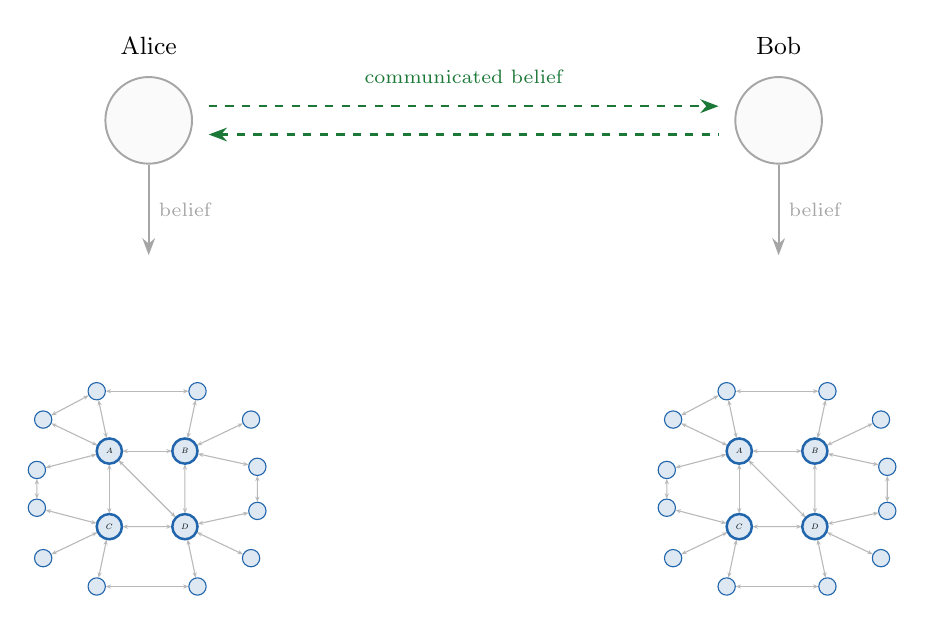
\begin{tikzpicture}
\node[agent] (al) at (0,0) {};
\node[font=\small] at (0,0.95) {Alice};
\mininet{L}{(-0.5,-4.2)}
\draw[->,gray!70,line width=0.7pt] (al.south) -- ++(0,-1.15)
      node[midway,right,font=\scriptsize]{belief};
\node[agent] (bo) at (8,0) {};
\node[font=\small] at (8,0.95) {Bob};
\mininet{R}{(7.5,-4.2)}
\draw[->,gray!70,line width=0.7pt] (bo.south) -- ++(0,-1.15)
      node[midway,right,font=\scriptsize]{belief};
\draw[->,dashed,social,line width=0.8pt] (al.east) ++(0.2,0.18)
      -- ($(bo.west)+(-0.2,0.18)$);
\draw[<-,dashed,social,line width=0.8pt] (al.east) ++(0.2,-0.18)
      -- ($(bo.west)+(-0.2,-0.18)$);
\node[social,font=\scriptsize] at (4,0.55) {communicated belief};
\end{tikzpicture}
\caption{\textbf{The setup.} Two agents each carry a belief over the
\emph{same} structured network of commitments and exchange those beliefs across
a trust channel (green, dashed). Within each network the four central nodes
$A,B,C,D$ (large) form the core; the surrounding nodes (small) are the
peripheral belt that touches observation. Links inside a network carry messages
in both directions (Figure~\ref{fig:anatomy}).}
\label{fig:setup}
\end{figure}

% =====================================================================
\section{The network and its updates: message passing}
% =====================================================================

Belief revision on the network is message passing. Each node takes input from
its neighbours and sends output back to them, so every link carries two
directed messages, one each way (Figure~\ref{fig:anatomy}). A node's belief is
revised by combining the evidence it receives with the messages arriving from
its neighbours; iterating this propagates a local change through the whole
structure. The core is simply the set of densely connected central commitments
through which most of these messages must pass.

\begin{figure}[t]
\centering
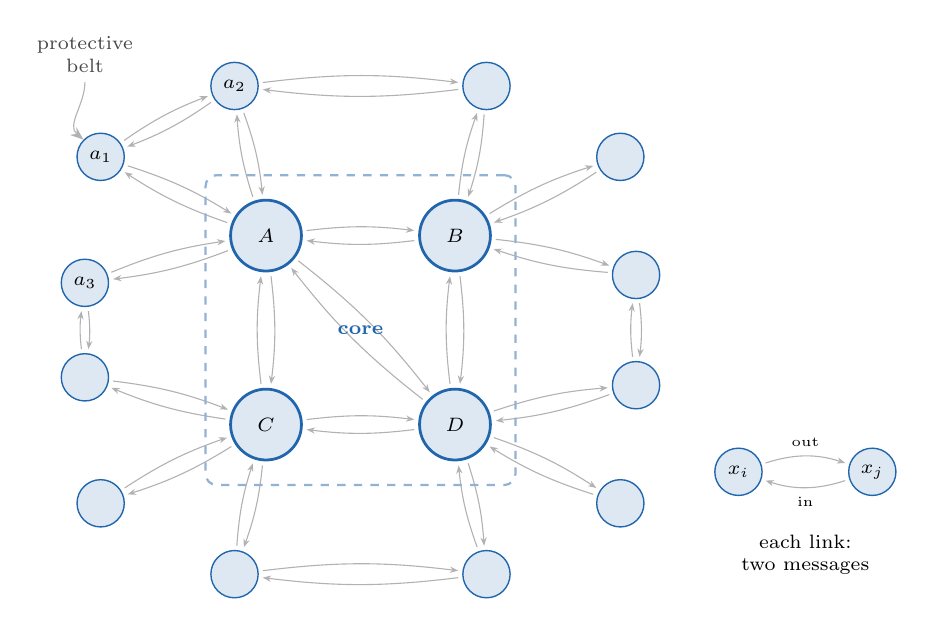
\begin{tikzpicture}
\beliefnetbase{core,old}{periph,old}
\begin{scope}[on background layer]
  \node[draw=paradA!50,dashed,rounded corners,line width=0.8pt,
        fit=(A)(B)(C)(D),inner sep=3mm] (corebox) {};
\end{scope}
\node[paradA,font=\scriptsize\bfseries] at (1.2,-1.2) {core};
\node[font=\scriptsize,align=center,gray!55!black] at (-2.3,2.3)
   {protective\\ belt};
\draw[->,gray!60] (-2.3,1.95) to[out=-90,in=140] (pA1.north west);
% --- inset: a single link = two opposed messages (input + output) ---
\begin{scope}[shift={(6.0,-3.0)}]
  \node[periph,old] (ni) at (0,0) {$x_i$};
  \node[periph,old] (nj) at (1.7,0) {$x_j$};
  \draw[msg] (ni) to[bend left=18] node[above,font=\tiny]{out} (nj);
  \draw[msg] (nj) to[bend left=18] node[below,font=\tiny]{in}  (ni);
  \node[font=\scriptsize,align=center] at (0.85,-1.05)
     {each link:\\ two messages};
\end{scope}
\end{tikzpicture}
\caption{\textbf{The network and message passing.} The same network, core
($A,B,C,D$) boxed. Every link carries two directed messages---input from a
neighbour and output to it (inset)---so revision is bidirectional propagation,
not a one-way flow. The core is the densely connected centre through which most
messages route; the belt is the network's sensory surface.}
\label{fig:anatomy}
\end{figure}

% =====================================================================
\section{Conservatism in the update setup}
% =====================================================================

Each node is revised by the motivated, tempered rule
$q'_i\propto q_{0,i}\,L_i^{\alpha/\lambda_i}\,e^{\,u_i/\lambda_i}$
\citep{hylandAlbarracin2025MindChange}, where $\lambda_i$ is the conservatism of
node $i$: the cost of moving its belief. The core/belt difference in this cost
is part of the update setup for the network, not a quantity read off the
graph. Central commitments are assigned higher $\lambda_i$ because much of the
network's interpretation rests on them---moving a core belief forces a great
deal of re-reading downstream---while peripheral beliefs are cheap to revise
(Figure~\ref{fig:conservatism}). The graded shading is this assigned
conservatism, the same gradient that will make the belt move before the core.

\begin{figure}[t]
\centering
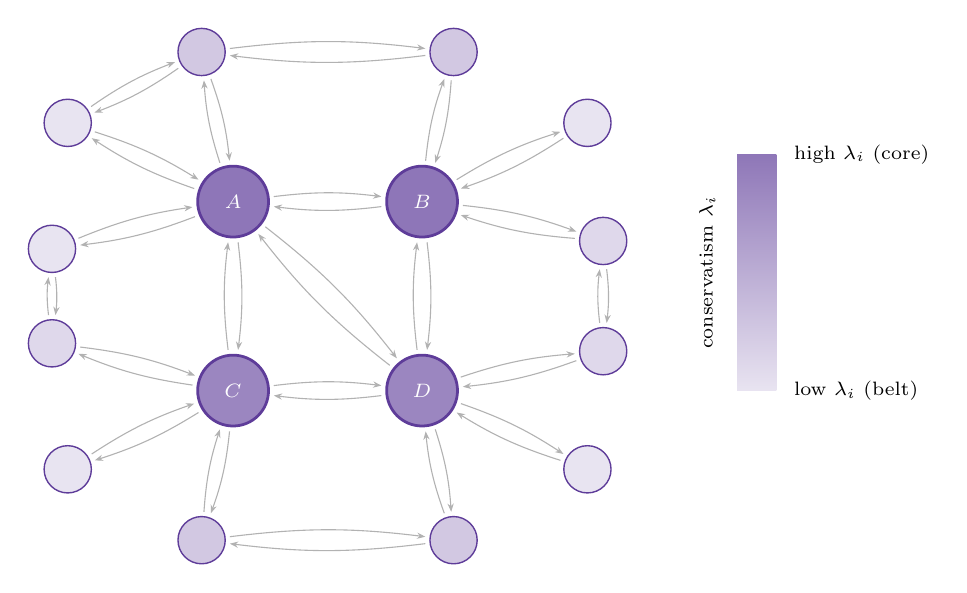
\begin{tikzpicture}
\foreach \n/\x/\y/\s in {A/0/0/70, B/2.4/0/70, C/0/-2.4/62, D/2.4/-2.4/62}
  {\node[core,draw=cons,fill=cons!\s,text=white] (\n) at (\x,\y) {$\n$};}
\foreach \n/\x/\y/\s in {%
   pA1/-2.1/1.0/14, pA2/-0.4/1.9/28, pA3/-2.3/-0.6/14,
   pB1/2.8/1.9/28, pB2/4.5/1.0/14, pB3/4.7/-0.5/20,
   pC1/-2.3/-1.8/20, pC2/-2.1/-3.4/14, pC3/-0.4/-4.3/28,
   pD1/2.8/-4.3/28, pD2/4.5/-3.4/14, pD3/4.7/-1.9/20}
  {\node[periph,draw=cons,fill=cons!\s] (\n) at (\x,\y) {};}
\begin{scope}[on background layer]
  \foreach \a/\b in \coreedges  {\biarrow{\a}{\b}}
  \foreach \a/\b in \periphedges{\biarrow{\a}{\b}}
  \foreach \a/\b in \crossedges {\biarrow{\a}{\b}}
\end{scope}
\begin{scope}[shift={(6.4,-2.4)}]
  \shade[bottom color=cons!14,top color=cons!70] (0,0) rectangle (0.5,3);
  \node[font=\scriptsize,anchor=west] at (0.6,3)   {high $\lambda_i$ (core)};
  \node[font=\scriptsize,anchor=west] at (0.6,0)   {low $\lambda_i$ (belt)};
  \node[font=\scriptsize,rotate=90,anchor=south] at (-0.15,1.5)
     {conservatism $\lambda_i$};
\end{scope}
\end{tikzpicture}
\caption{\textbf{Conservatism in the update setup.} Shade encodes $\lambda_i$,
the cost of revising node $i$. Central commitments (dark) are assigned higher
conservatism than peripheral ones (light), because much of the network's
interpretation rests on them. This assignment is part of how the network is set
up to update; it is not derived from the directed structure of the graph.}
\label{fig:conservatism}
\end{figure}

% =====================================================================
\section{Belief-utility concentrates on the core}
% =====================================================================

Conservatism $\lambda_i$ is a \emph{symmetric} stiffness---it resists motion in
any direction. The affective belief-utility $u_i$ is \emph{directional}---it
pulls the belief toward a preferred value regardless of evidence. The two are
distinct costs that look alike in a single update but separate when evidence is
sparse or when prior and preference disagree. Like conservatism, $u_i$ is
naturally concentrated on the core: agents have no feelings about which
peripheral bookkeeping is correct, but strong commitments about the central
claims (Figure~\ref{fig:utility}). Conservatism gives convergence at varying
speeds; a supra-threshold core $u_i$ is what can produce permanent lock-in even
as evidence accumulates.

\begin{figure}[t]
\centering
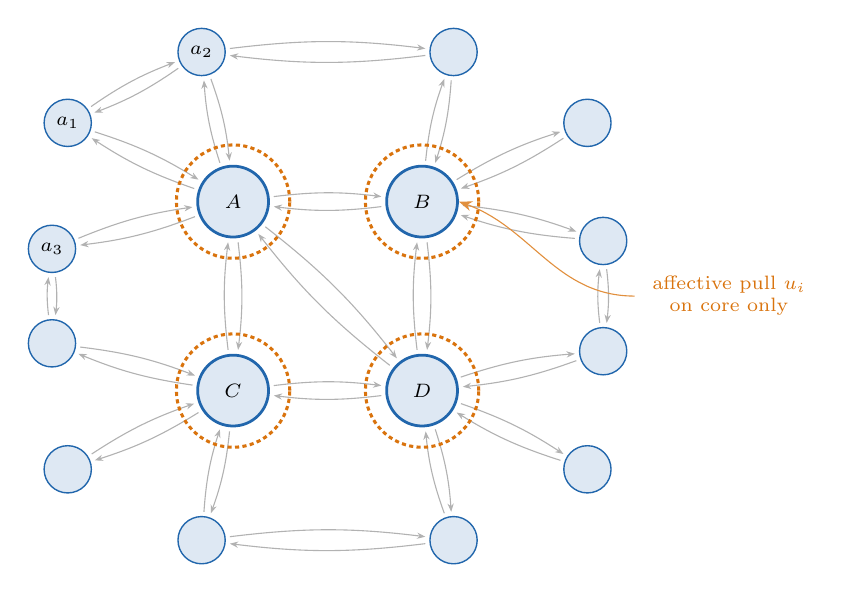
\begin{tikzpicture}
\beliefnetbase{core,old}{periph,old}
\foreach \n in {A,B,C,D}
  {\draw[util,line width=1.1pt,dash pattern=on 1.5pt off 1.2pt]
     (\n) circle (7.2mm);}
\node[util,font=\scriptsize,align=center,anchor=west] at (5.2,-1.2)
   {affective pull $u_i$\\ on core only};
\draw[->,util!80] (5.1,-1.2) to[out=180,in=-20] (B.east);
\end{tikzpicture}
\caption{\textbf{Belief-utility on the core.} Orange haloes mark nodes with
nonzero affective utility $u_i$: a preference for a particular value of the
central commitments, independent of fit. The belt is affectively neutral. The
update $q'_i\propto q_{0,i}L_i^{\alpha/\lambda_i}e^{u_i/\lambda_i}$ runs
node-wise; only the core carries the $e^{u_i/\lambda_i}$ tilt.}
\label{fig:utility}
\end{figure}

% =====================================================================
\section{Evidence enters the belt and propagates inward}
% =====================================================================

An observation is evidentially connected to peripheral nodes. It updates them
near-Bayesianly, because their $\lambda_i$ is low, and message passing then
carries the implication inward. As it advances toward the core the conservatism
it meets rises, so the update slows (Figure~\ref{fig:propagation}). This is the
gradient that produces the dynamics of the next section: evidence diffuses
inward but is increasingly resisted, and the core moves only once enough of the
belt has been re-interpreted.

\begin{figure}[t]
\centering
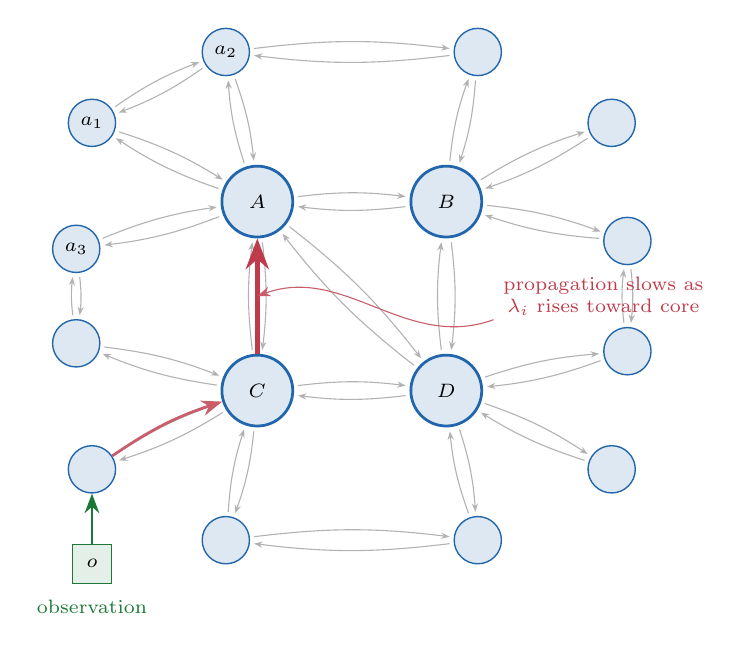
\begin{tikzpicture}
\beliefnetbase{core,old}{periph,old}
\node[obsq] (o) at (-2.1,-4.6) {$o$};
\draw[->,social,line width=0.9pt] (o) -- (pC2);
\draw[->,paradB!70,line width=1.0pt] (pC2) to[bend left=8] (C);
\draw[->,paradB!85,line width=1.8pt] (C) -- (A);
\node[font=\scriptsize,social] at (-2.1,-5.15) {observation};
\node[font=\scriptsize,align=center,paradB!85,anchor=west] at (3.0,-1.2)
   {propagation slows as\\ $\lambda_i$ rises toward core};
\draw[->,paradB!70] (3.0,-1.5) to[out=200,in=20] ($(A)!0.5!(C)$);
\end{tikzpicture}
\caption{\textbf{Inward propagation against rising conservatism.} An observation
$o$ (green) enters at a leaf and flips it cheaply. Its implication propagates
inward (red), but each step toward the core meets higher $\lambda_i$
(thickening arrow = greater resistance). Peripheral nodes track the data; the
core lags.}
\label{fig:propagation}
\end{figure}

% =====================================================================
\section{The paradigm shift as a percolation cascade}
% =====================================================================

Run the dynamics and a characteristic signature appears. For a long time only
the belt moves: peripheral nodes flip to the new paradigm one by one as evidence
accumulates, while the core holds. Each flip removes some of the inferential
support the core relied on. Once enough of the belt has been hollowed out, the
core can no longer be sustained against the evidence, and it gives way
\emph{together}, quickly---a percolation-like cascade
(Figure~\ref{fig:cascade}). The macroscopic appearance is exactly Kuhn's: long
stability with visible activity only at the edges, then a sudden reorganisation.
The discrete-$\theta$ model could not produce this, because it had no internal
structure for a transition to propagate through.

\begin{figure}[t]
\centering
\newcommand{\panel}[1]{% #1 = comma list of nodes already flipped to "new"
  \begin{tikzpicture}[scale=0.52,transform shape]
    \beliefnetbase{core,old}{periph,old}
    \foreach \n in {#1}{%
       \node[circle,inner sep=0pt,draw=paradB,fill=paradB!22,
             minimum size=6mm,line width=0.5pt] at (\n) {};}
  \end{tikzpicture}}
\begin{minipage}{0.32\textwidth}\centering
  \panel{pA1,pC2}\\[2pt]
  {\footnotesize (a) $t_1$: belt erosion begins}
\end{minipage}\hfill
\begin{minipage}{0.32\textwidth}\centering
  \panel{pA1,pA2,pA3,pB2,pC1,pC2,pC3,pD2}\\[2pt]
  {\footnotesize (b) $t_2$: belt hollowed, core holds}
\end{minipage}\hfill
\begin{minipage}{0.32\textwidth}\centering
  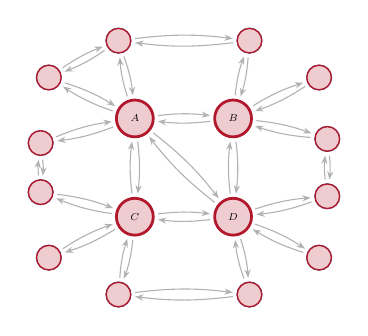
\begin{tikzpicture}[scale=0.52,transform shape]
    \beliefnetbase{core,new}{periph,old}
    \foreach \n in {pA1,pA2,pA3,pB1,pB2,pB3,pC1,pC2,pC3,pD1,pD2,pD3}{%
       \node[circle,inner sep=0pt,draw=paradB,fill=paradB!22,
             minimum size=6mm,line width=0.5pt] at (\n) {};}
  \end{tikzpicture}\\[2pt]
  {\footnotesize (c) $t_3$: core cascades}
\end{minipage}
\caption{\textbf{Percolation cascade = phase shift.} Blue is the old paradigm,
red the new. (a)~A few peripheral nodes flip cheaply. (b)~Evidence has converted
most of the belt, but the high-$\lambda$ core still resists---the long quiet
period, with activity only at the edges. (c)~With the belt's support gone the
core can no longer be defended and flips as a block. The transition is gradual
at the periphery and sudden at the centre.}
\label{fig:cascade}
\end{figure}

% =====================================================================
\section{Communicating a changed mind}
% =====================================================================

Suppose the cascade runs in Alice: her belief over the network has moved, core
and belt, to the new paradigm. She must now convey this to Bob across the trust
channel. With a scalar $\theta$ the message was simply a posterior over $K$
values. With a structured belief the message is a structured object, and it is
no longer obvious \emph{what} should be sent (Figure~\ref{fig:communication}).
She could transmit only the node marginals $\{q(x_i)\}$---cheap, but discarding
the correlations that made her change coherent; the full joint
$q(x_1,\dots,x_n)$---exact, and for a small network entirely feasible to send;
or a set of factor fragments, conditional bundles such as ``if $A$ then $B$
because $C$''---the form closest to how scientific claims are actually
communicated. The choice fixes how much of Alice's reorganisation survives in
Bob, and so how the cascade spreads through the population. We take it as an
open modelling question rather than settling it here; for a small network the
joint is the natural default, with fragments the more realistic refinement.

\begin{figure}[t]
\centering
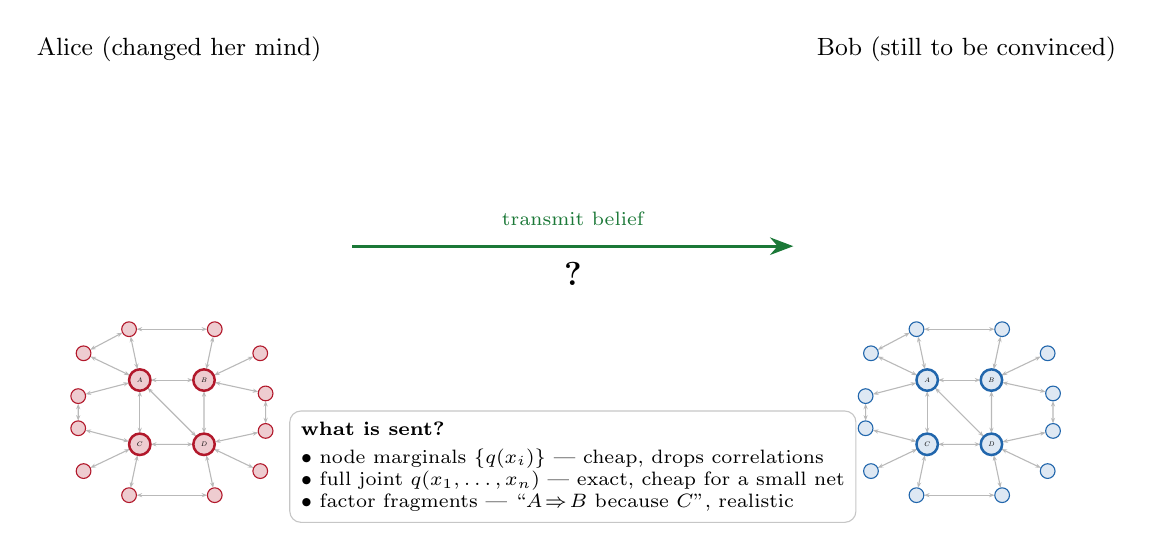
\begin{tikzpicture}
% --- Alice: changed her mind (all red) ---
\node[font=\small] at (0,2.3) {Alice (changed her mind)};
\begin{scope}[shift={(-0.5,-1.9)},scale=0.34,transform shape]
  \foreach \n/\x/\y in \corelist
    {\node[bnode,new,minimum size=8mm,line width=0.9pt] (a\n) at (\x,\y) {$\n$};}
  \foreach \n/\x/\y/\lab in \periphlist
    {\node[bnode,new,minimum size=5.5mm] (a\n) at (\x,\y) {};}
  \begin{scope}[on background layer]
    \foreach \p/\q in \coreedges  {\draw[minilink] (a\p)--(a\q);}
    \foreach \p/\q in \periphedges{\draw[minilink] (a\p)--(a\q);}
    \foreach \p/\q in \crossedges {\draw[minilink] (a\p)--(a\q);}
  \end{scope}
\end{scope}
% --- Bob: still old (all blue) ---
\node[font=\small] at (10,2.3) {Bob (still to be convinced)};
\begin{scope}[shift={(9.5,-1.9)},scale=0.34,transform shape]
  \foreach \n/\x/\y in \corelist
    {\node[bnode,old,minimum size=8mm,line width=0.9pt] (b\n) at (\x,\y) {$\n$};}
  \foreach \n/\x/\y/\lab in \periphlist
    {\node[bnode,old,minimum size=5.5mm] (b\n) at (\x,\y) {};}
  \begin{scope}[on background layer]
    \foreach \p/\q in \coreedges  {\draw[minilink] (b\p)--(b\q);}
    \foreach \p/\q in \periphedges{\draw[minilink] (b\p)--(b\q);}
    \foreach \p/\q in \crossedges {\draw[minilink] (b\p)--(b\q);}
  \end{scope}
\end{scope}
% --- the channel and the open question ---
\draw[->,social,line width=1.2pt] (2.2,-0.2) -- (7.8,-0.2);
\node[social,font=\scriptsize] at (5,0.15) {transmit belief};
\node[font=\large] at (5,-0.55) {\textbf{?}};
\node[draw=gray!45,rounded corners,align=left,font=\scriptsize,
      inner sep=4pt] at (5,-3.0)
  {\textbf{what is sent?}\\[2pt]
   $\bullet$ node marginals $\{q(x_i)\}$ --- cheap, drops correlations\\
   $\bullet$ full joint $q(x_1,\dots,x_n)$ --- exact, cheap for a small net\\
   $\bullet$ factor fragments --- ``$A\!\Rightarrow\!B$ because $C$'', realistic};
\end{tikzpicture}
\caption{\textbf{Communicating a changed mind.} After the cascade, Alice's whole
network has moved to the new paradigm (red); Bob's has not (blue). To convey her
new belief she must choose what to transmit: node marginals (cheap, lossy), the
full joint (exact, and feasible for a small network), or factor fragments
(claims with their inferential support, closest to real scientific
communication). The choice determines how much of her reorganisation survives in
Bob---an open question the scalar model never had to face.}
\label{fig:communication}
\end{figure}

% =====================================================================
\section{The macroscopic signature}
% =====================================================================

Aggregating over the population gives the order parameters to measure. The mean
peripheral belief drifts down smoothly as evidence converts the belt; the mean
core belief stays near its prior, then drops sharply once the percolation
threshold is crossed (Figure~\ref{fig:signature}a). Across the coupled
population, with one-round transmission delays, the approach to the new
consensus is a damped oscillation whose damping is set by the distribution of
conservatism $\{\lambda_i\}$ and the spectral structure of the trust matrix
(Figure~\ref{fig:signature}b). The curves are illustrative schematics of the
target phenomenology, not simulation output.

\begin{figure}[t]
\centering
\begin{minipage}{0.49\textwidth}\centering
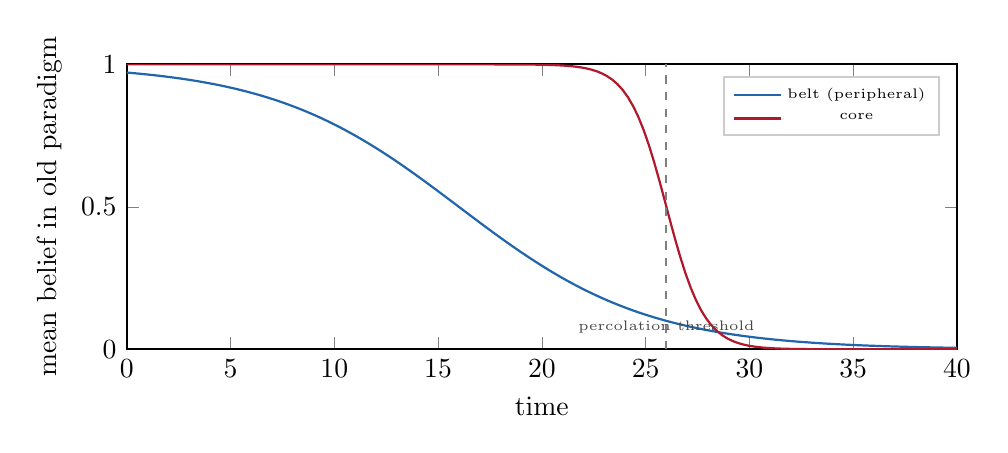
\begin{tikzpicture}
\begin{axis}[width=\textwidth,height=5.2cm,
  xlabel={time}, ylabel={mean belief in old paradigm},
  xmin=0,xmax=40,ymin=0,ymax=1,ytick={0,0.5,1},
  legend style={font=\tiny,at={(0.98,0.96)},anchor=north east,draw=gray!40},
  domain=0:40,samples=160,thick,every axis plot/.append style={line width=0.8pt}]
\addplot[paradA]{1-1/(1+exp(-0.22*(x-16)))};
\addlegendentry{belt (peripheral)}
\addplot[paradB]{1-1/(1+exp(-1.1*(x-26)))};
\addlegendentry{core}
\draw[gray,dashed] (axis cs:26,0)--(axis cs:26,1);
\node[font=\tiny,anchor=south,gray!55!black] at (axis cs:26,0.02)
   {percolation threshold};
\end{axis}
\end{tikzpicture}\\[2pt]
{\footnotesize (a) gradual belt drift, sudden core flip}
\end{minipage}\hfill
\begin{minipage}{0.49\textwidth}\centering
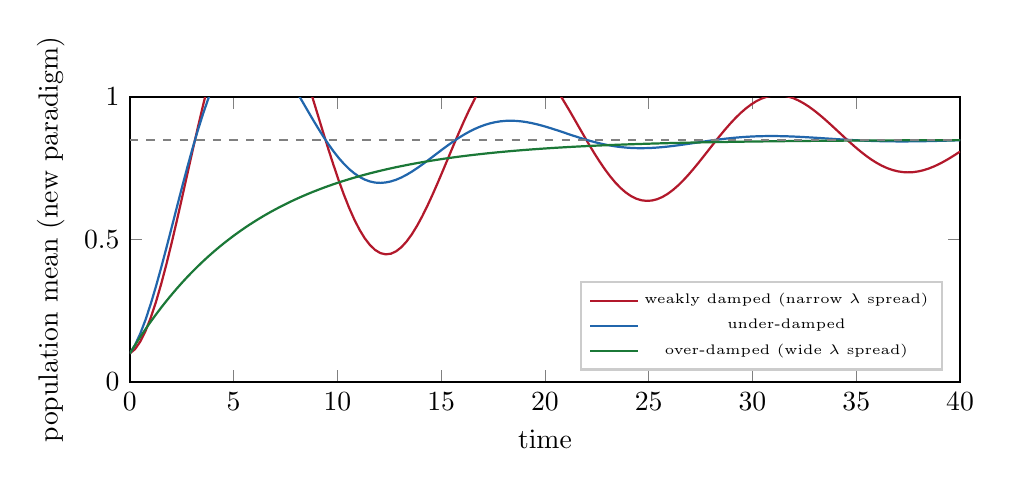
\begin{tikzpicture}
\begin{axis}[width=\textwidth,height=5.2cm,
  xlabel={time}, ylabel={population mean (new paradigm)},
  xmin=0,xmax=40,ymin=0,ymax=1,ytick={0,0.5,1},
  legend style={font=\tiny,at={(0.98,0.04)},anchor=south east,draw=gray!40},
  domain=0:40,samples=160,thick,every axis plot/.append style={line width=0.8pt}]
\addplot[paradB]{0.85-0.75*exp(-0.05*x)*cos(deg(0.5*x))};
\addlegendentry{weakly damped (narrow $\lambda$ spread)}
\addplot[paradA]{0.85-0.75*exp(-0.13*x)*cos(deg(0.5*x))};
\addlegendentry{under-damped}
\addplot[social]{0.85-0.75*exp(-0.16*x)};
\addlegendentry{over-damped (wide $\lambda$ spread)}
\draw[gray,dashed] (axis cs:0,0.85)--(axis cs:40,0.85);
\end{axis}
\end{tikzpicture}\\[2pt]
{\footnotesize (b) approach to consensus vs.\ $\{\lambda_i\}$}
\end{minipage}
\caption{\textbf{Macroscopic signature (schematic; not simulation output).}
(a)~The mean peripheral belief drifts smoothly while the mean core belief holds,
then drops sharply at the percolation threshold (dashed)---the order-parameter
form of a Kuhnian phase shift. (b)~Coupled through the trust network with
transmission delay, the population approaches the new consensus as a damped
oscillation whose regime is governed by the distribution of conservatism and the
spectrum of the trust matrix.}
\label{fig:signature}
\end{figure}

% =====================================================================
\section*{Outlook}
% =====================================================================
\addcontentsline{toc}{section}{Outlook}

Structuring the paradigm turns the phase-shift signature into a consequence
rather than an assumption: it is a percolation cascade through a network whose
core is held by the conservatism of the update setup. It also raises a question
the scalar model could not pose---once a mind has changed, what is communicated:
marginals, the joint, or inferential fragments. The same machinery is invariant
under a change of who controls attention over the network: in science, attention
is shaped by the agent and its community; in algorithmically curated settings it
is shaped externally, and beliefs propagate by salience rather than by
trust---the formal object is the same, the generator of the attention
distribution is not.

\begin{thebibliography}{9}
\bibitem[Albarracin et al.(2022)]{albarracin2022EpistemicCommunities}
M.~Albarracin, D.~Demekas, M.~J.~D.~Ramstead, and C.~Heins.
\newblock Epistemic Communities under Active Inference.
\newblock \emph{Entropy}, 24(4):476, 2022.

\bibitem[Hyland and Albarracin(2025)]{hylandAlbarracin2025MindChange}
D.~Hyland and M.~Albarracin.
\newblock On the Variational Costs of Changing Our Minds.
\newblock \emph{arXiv preprint} arXiv:2509.17957, 2025.

\bibitem[Kuhn(1962)]{kuhn1962Structure}
T.~S.~Kuhn.
\newblock \emph{The Structure of Scientific Revolutions}.
\newblock University of Chicago Press, 1962.

\bibitem[Lakatos(1970)]{lakatos1970Methodology}
I.~Lakatos.
\newblock Falsification and the methodology of scientific research programmes.
\newblock In \emph{Criticism and the Growth of Knowledge}. Cambridge UP, 1970.
\end{thebibliography}

\end{document}
